\begin{figure}[htbp]
\section*{ FBXL4}
\centering
\begin{subfigure}[b]{0.95\textwidth}
\centering
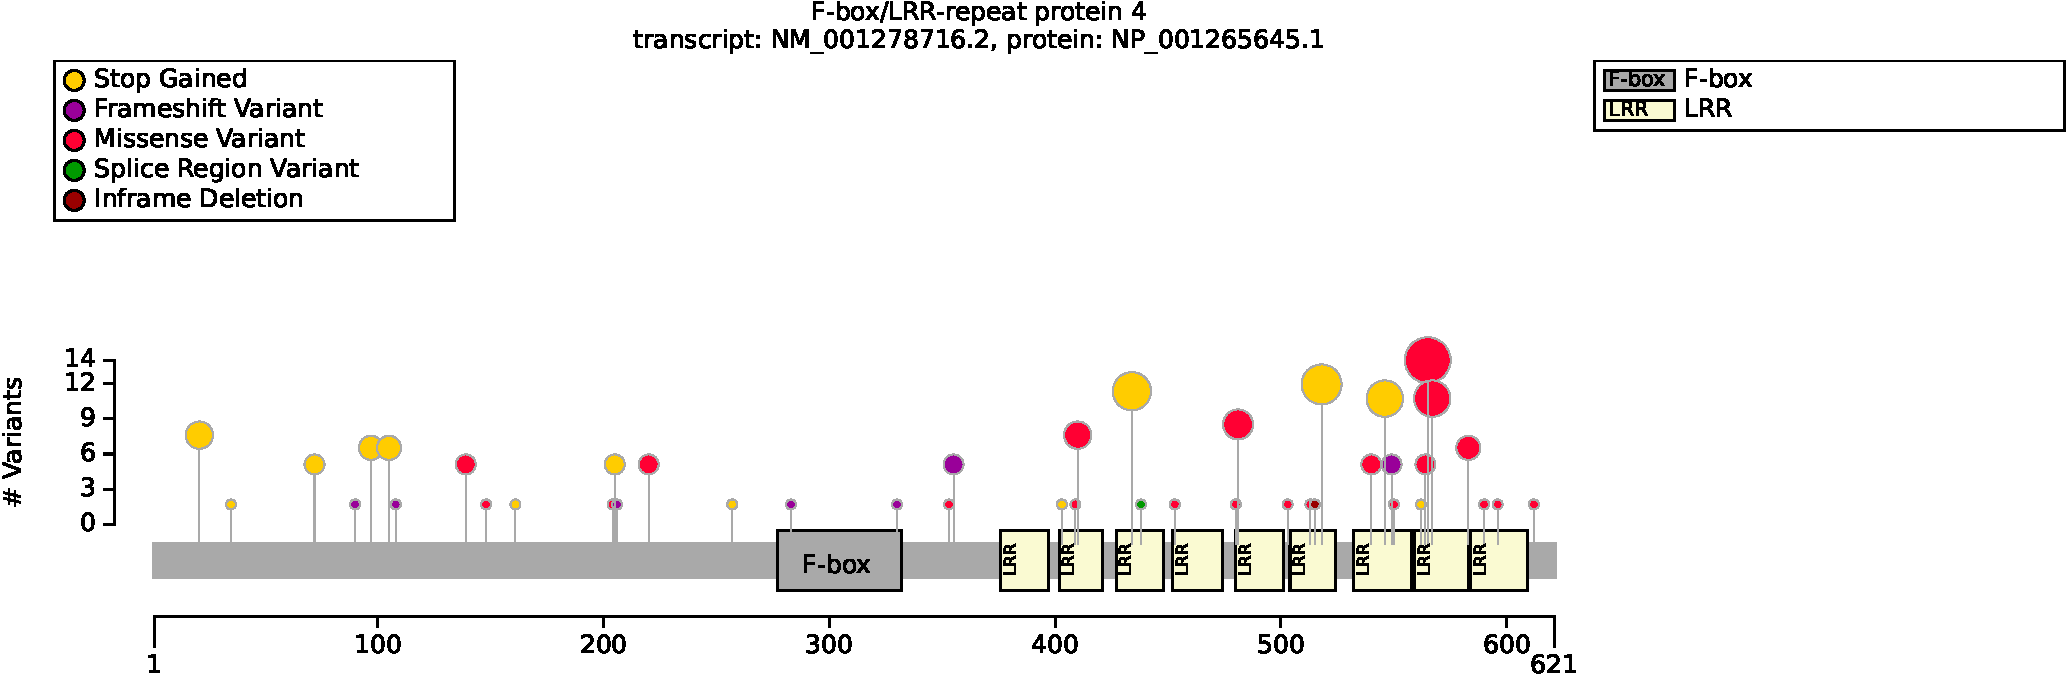
\includegraphics[width=\textwidth]{ img/FBXL4_protein_diagram.pdf} 
\captionsetup{justification=raggedright,singlelinecheck=false}
\caption{Distribution of variants in FBXL4}
\end{subfigure}

\vspace{2em}

\begin{subfigure}[b]{0.95\textwidth}
\centering
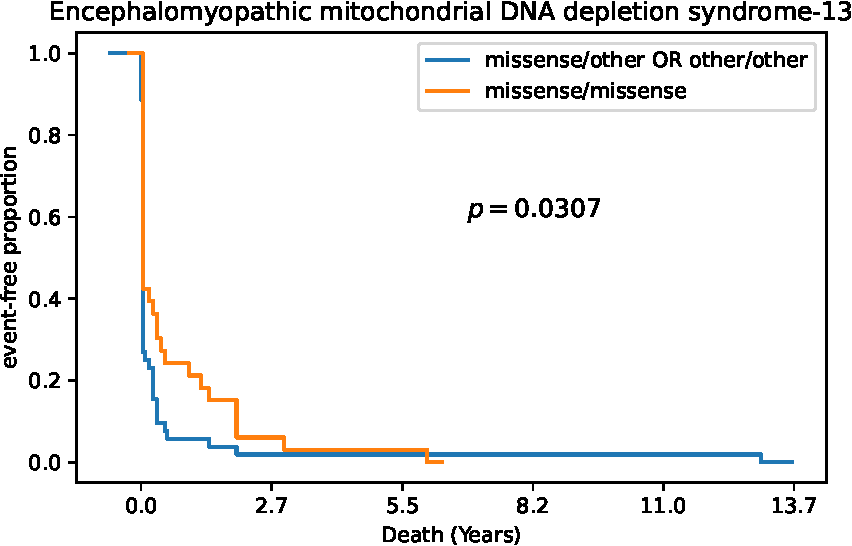
\includegraphics[width=0.3\textwidth]{ img/FBXL4_stats.pdf} 
\captionsetup{justification=raggedright,singlelinecheck=false}
\caption{Survival analysis.}
\end{subfigure}

\vspace{1em}

\begin{subfigure}[b]{0.95\textwidth}
\centering
\resizebox{\textwidth}{!}{
\begin{tabular}{llllrr}
\toprule
HPO term & missense/other OR other/other & missense/missense & p-value & adj. p-value\\
\midrule
Feeding difficulties [HP:0011968] & 23/24 (96\%) & 13/27 (48\%) & $1.73\times 10^{-4}$ & 0.004\\
\bottomrule
\end{tabular}
}
\captionsetup{justification=raggedright,singlelinecheck=false}
\caption{Fisher Exact Test performed to compare HPO annotation frequency with respect to missense/other OR other/other and missense/missense. Total of
        22 tests were performed.}
\end{subfigure}
\vspace{2em}
\begin{subfigure}[b]{0.95\textwidth}
\centering
\resizebox{\textwidth}{!}{
\begin{tabular}{llllrr}
\toprule
Genotype (A) & Genotype (B) & total tests performed & significant results\\
\midrule
LRR domain/LRR domain OR LRR domain/other & other/other & 24 & 0\\
LRR domain/LRR domain OR LRR domain/other & other/other & 24 & 0\\
FEMALE & MALE & 21 & 0\\
\bottomrule
\end{tabular}
}
\captionsetup{justification=raggedright,singlelinecheck=false}
\caption{Fisher Exact Test performed to compare HPO annotation frequency with respect to genotypes.}
\end{subfigure}


\begin{subfigure}[b]{0.95\textwidth}
\captionsetup{justification=raggedright,singlelinecheck=false}
\resizebox{\textwidth}{!}{
\begin{tabular}{llllrr}
\toprule
Description & Variable & Genotype (A) & Genotype (B) & p-value & xrefs\\
\midrule
Compute time until OMIM:615471 onset & Onset of OMIM:615471 & missense/other OR other/other & missense/missense & 0.031 & -\\
Compute time until postnatal death & Age of death & missense/other OR other/other & missense/missense & 0.080 & -\\
\bottomrule
\end{tabular}
}
\caption{Survival analysis for Age of death and onset, comparing compare missense/other OR other/other and missense/missense. }
\end{subfigure}


\caption{The cohort comprised 95 individuals (37 females, 58 males). 26 of these individuals were reported to be deceased. 
A total of 91 HPO terms were used to annotate the cohort. Disease diagnosis: Mitochondrial DNA depletion syndrome 13 (encephalomyopathic type)
 (OMIM:615471). It was reported that  pathological variants in FBXL4 indicated that genotypes with 
 missense variants are frequently associated with longer survival \cite{PMID_28940506}. Using the larger cohort analyzed here, mortality is not significantly associated with 
 missense variants (p-value 0.08), but there was a significant association with age of onset (being later for missense variants).
 A total of 117 unique variant alleles were found in \textit{FBXL4} (transcript: \texttt{NM\_001278716.2}, protein id: \texttt{NP\_001265645.1}).}
\end{figure}
